\section{Experimental Results}
\subsection{Tweet Data Collection and Processing}
\subsubsection{Processed dataset structure}
\begin{figure}[h]
\centering
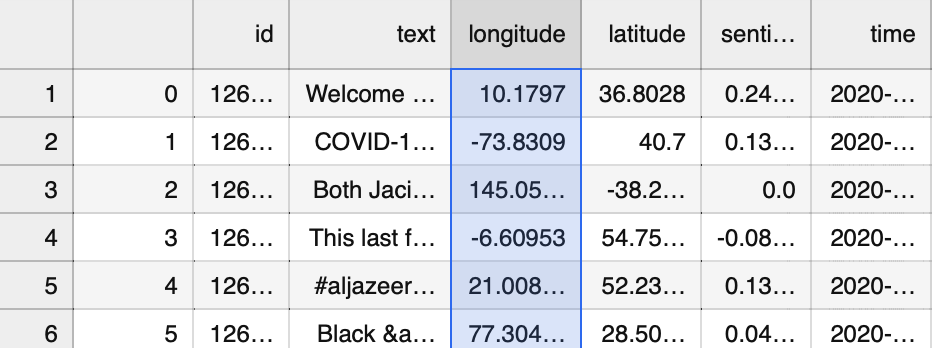
\includegraphics[width=0.5\textwidth]{imgs/tweets structure.png}
\caption{\label{fig:Research process}Completed dataset}
\end{figure}
The file above  shows the result of Tweet Date Collection. It will be store in
a corresponding CSV file. Then we read each file and import the data into the
elasticsearch server (Fig.8).
\begin{figure}[h]
\centering
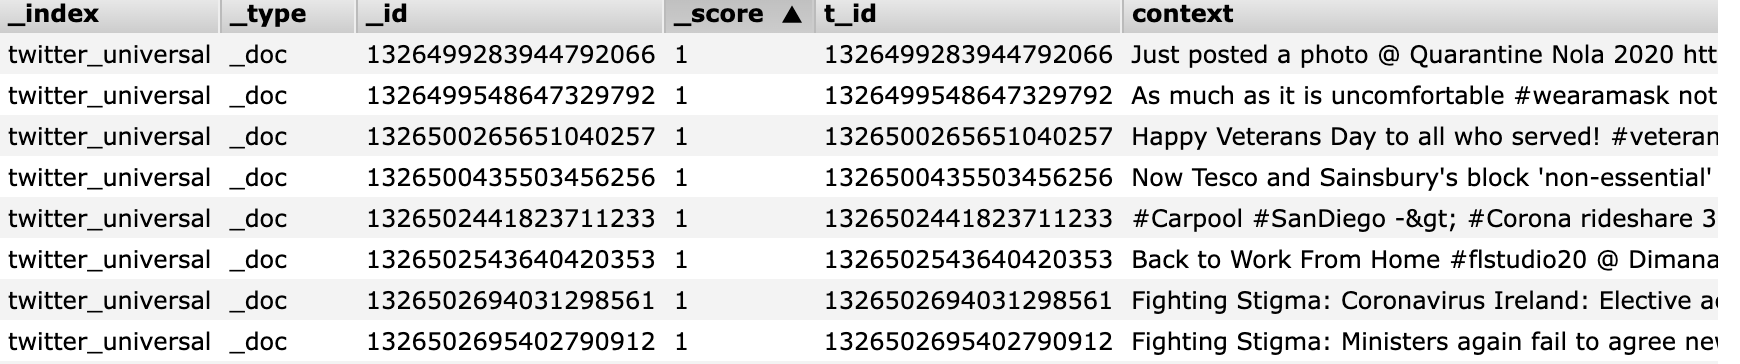
\includegraphics[width=0.5\textwidth]{imgs/es_result.png}
\caption{\label{fig:Research process}Data in elasticsearch}
\end{figure}
Then we apply the pre-processing program on the dataset. Shows the result of words dataset (Fig.9). 

\subsection{Topic Clustering}
After training on a filtered subset of the dataset, we get the topic cluster shown in (Fig.10) below: 
    \begin{figure}[H]
        \centering
        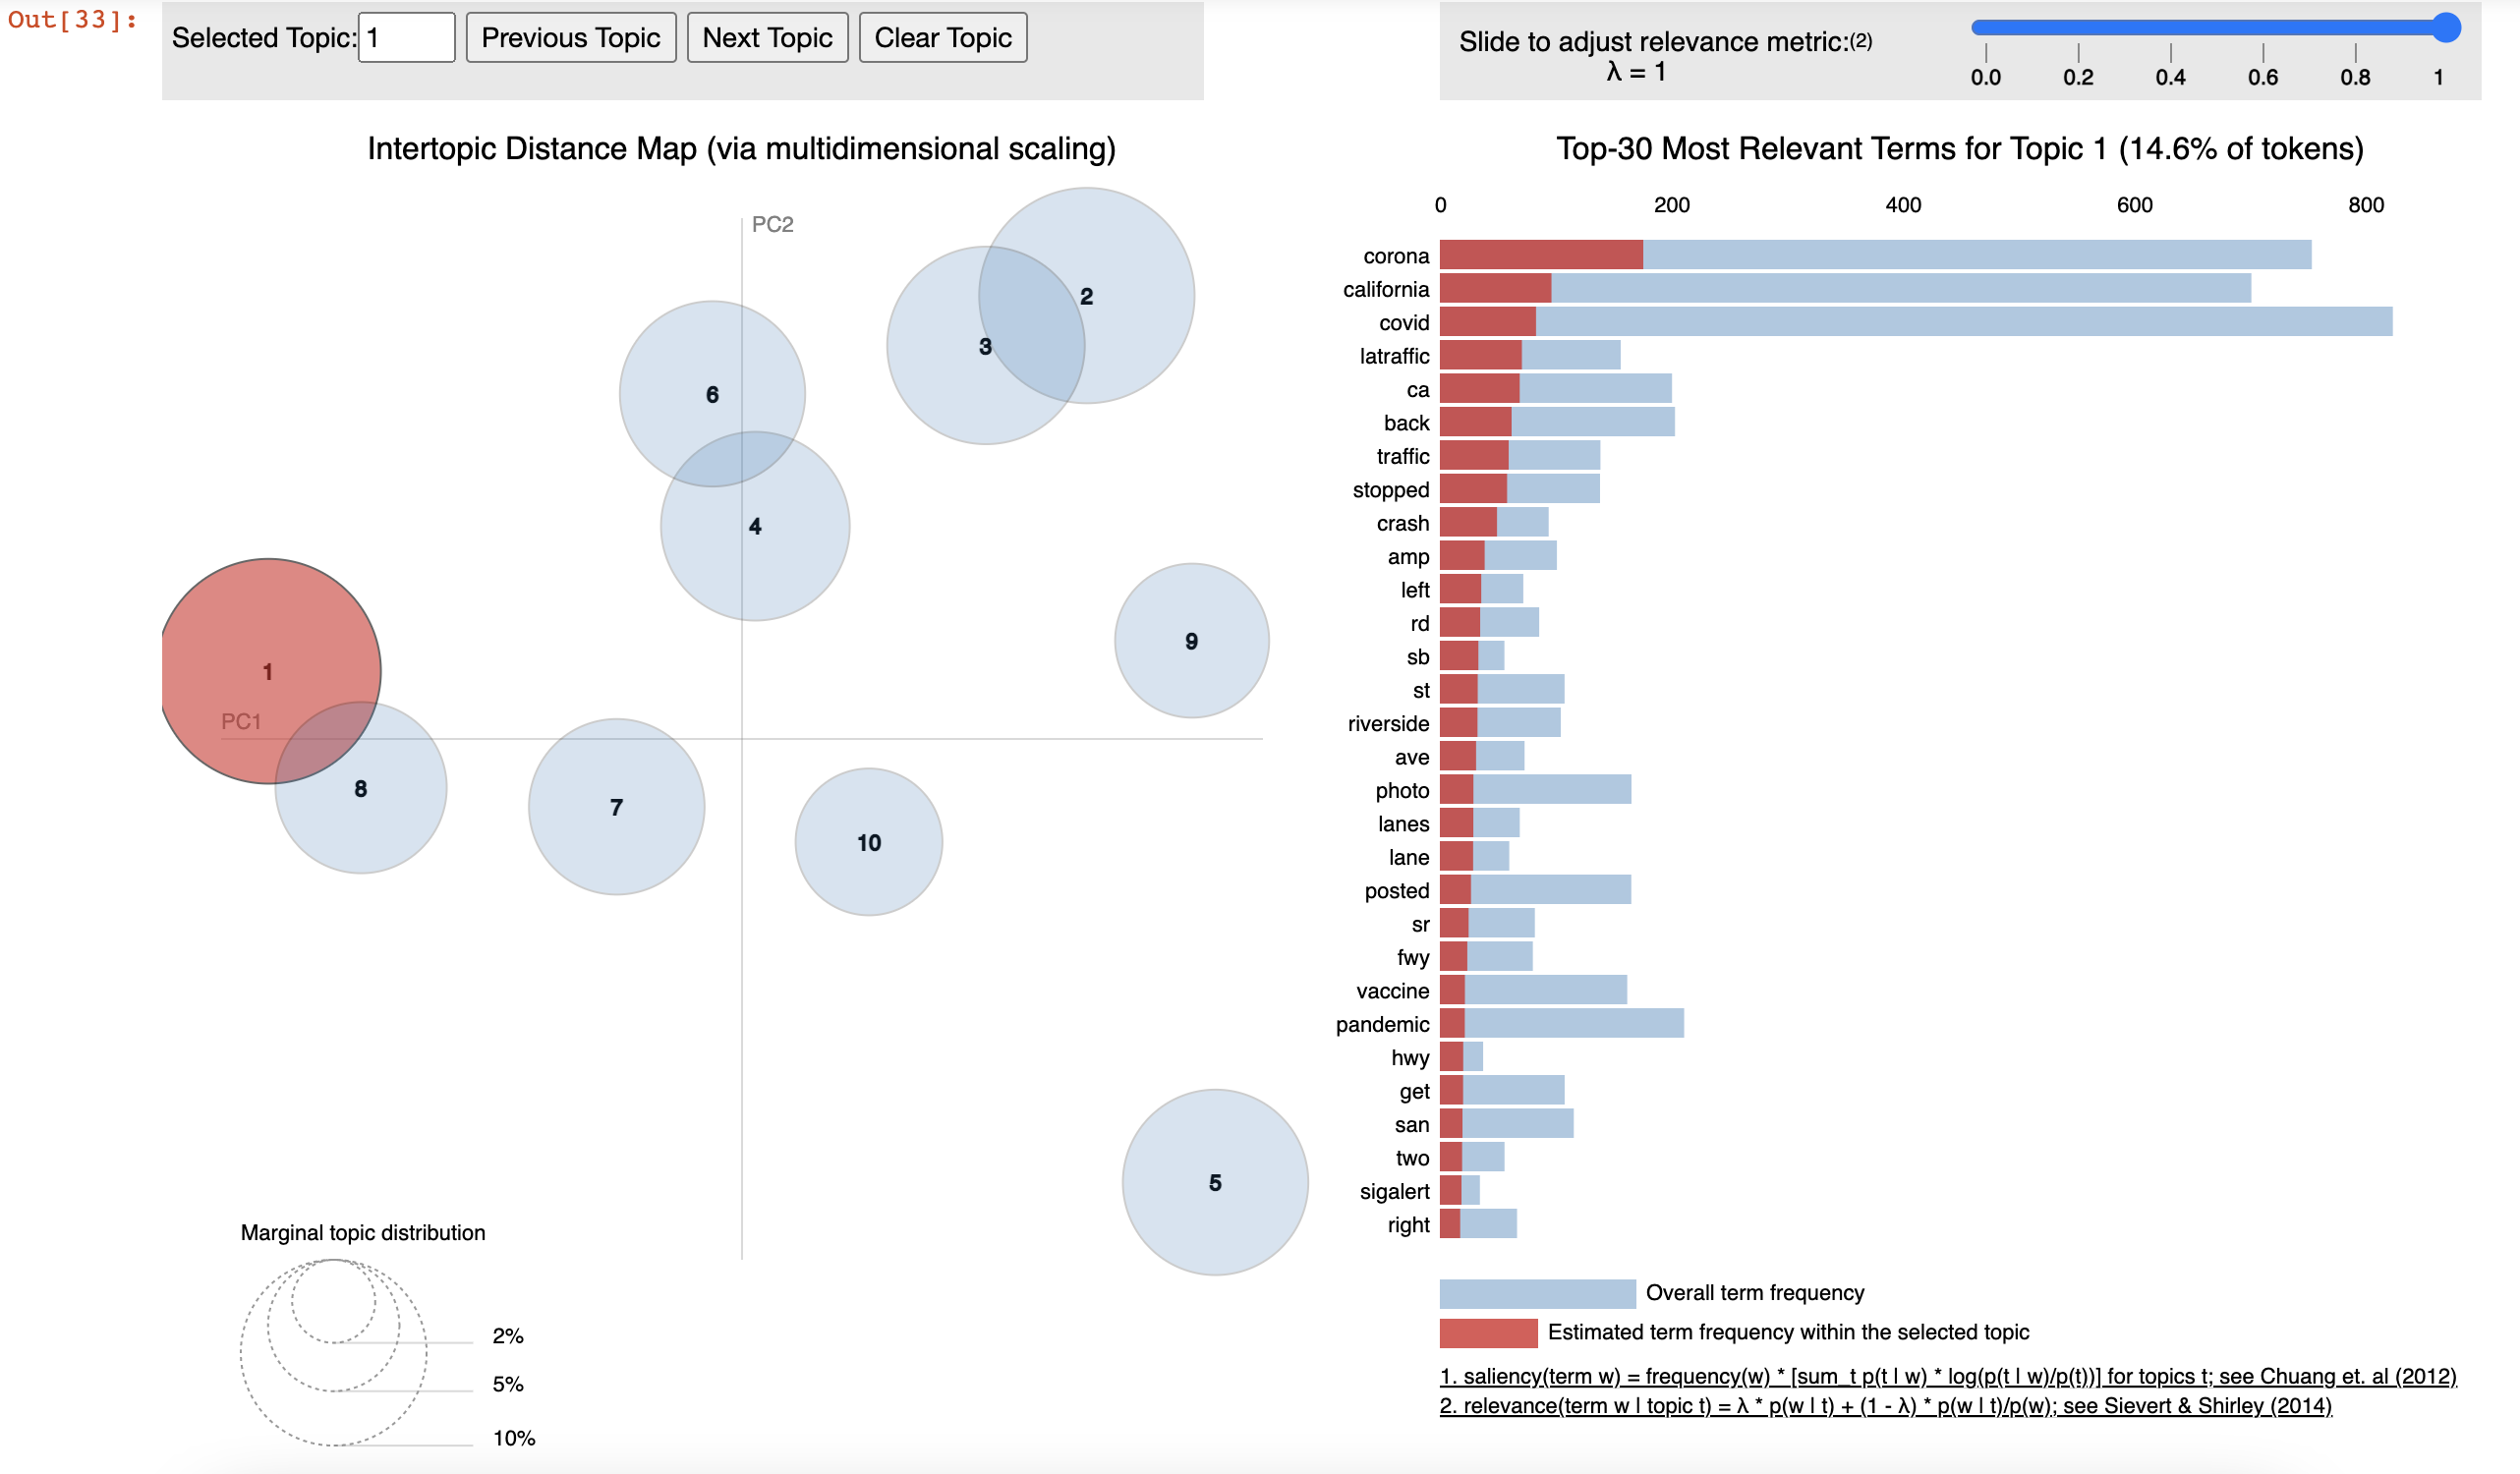
\includegraphics[width=0.5\textwidth]{imgs/cluster_topics.png}
        \caption{Topic Clusters produced using LDA}
        \label{fig:lda_topic}
    \end{figure}
For demonstration, we show the term distribution and rank of topic cluster 1
from the trained model which has been visualized using pyLDAViz library in
(Fig.11):
\begin{figure}[H]
    \centering
    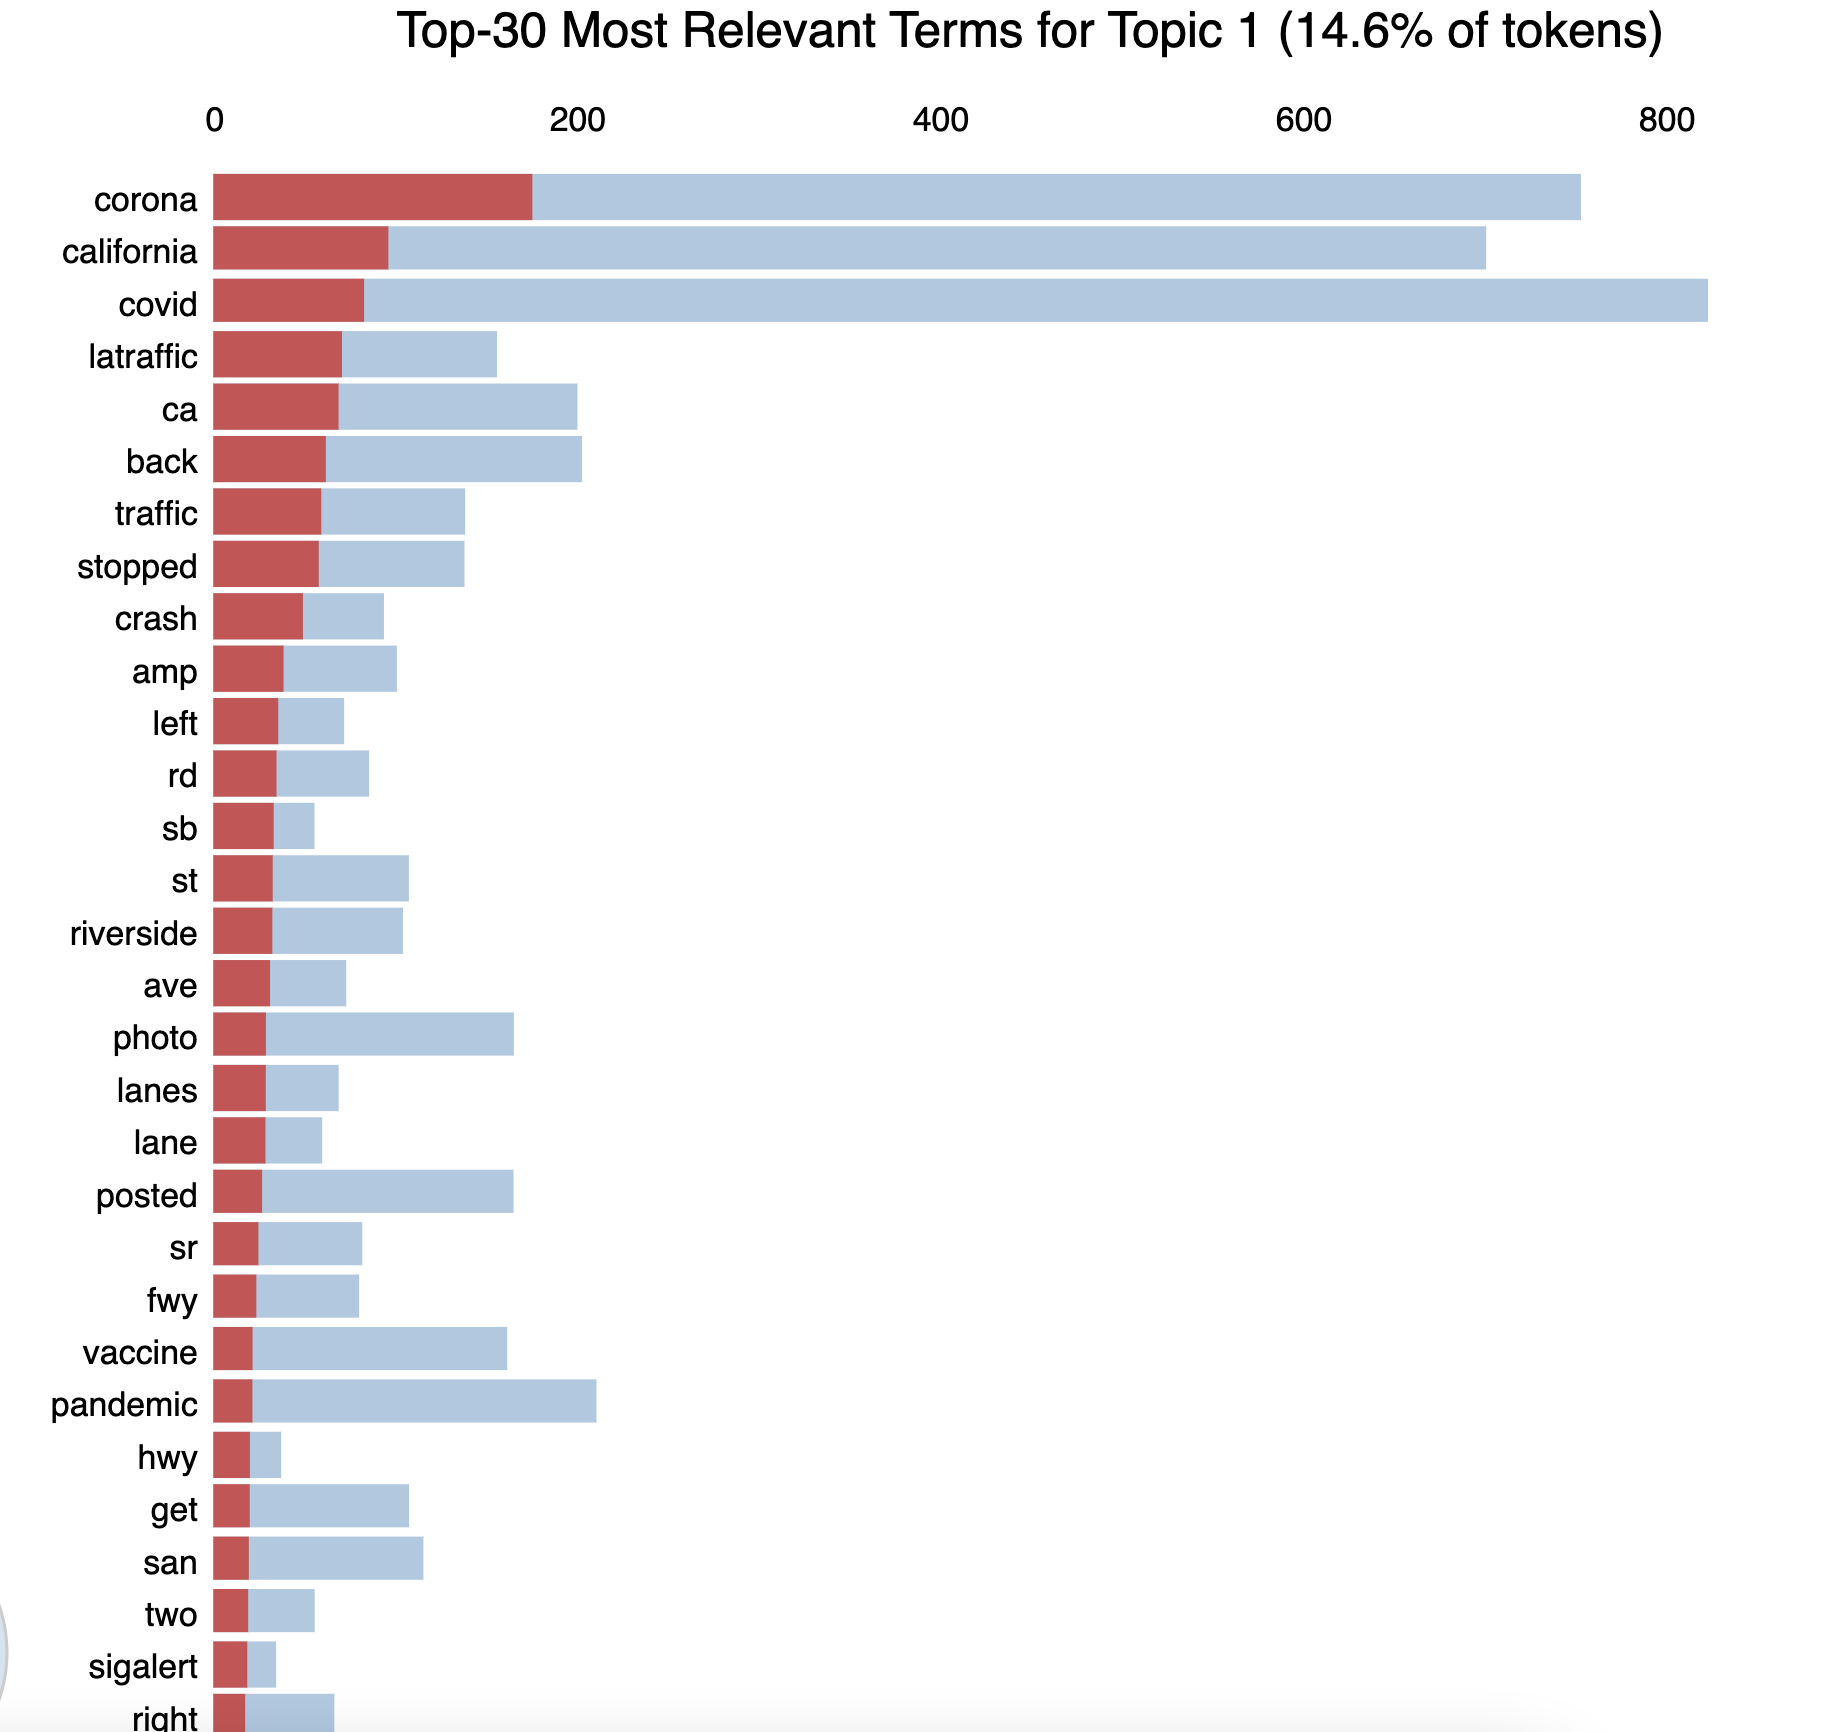
\includegraphics[width=0.5\textwidth]{imgs/term_ranks.png}
    \caption{Rank of Terms in Cluster 1}
    \label{fig:my_label}
\end{figure}
For testing the trained model, we have taken samples from unseen data and used
inference technique to find out the topic probability distribution for those
samples. In the example below, for demonstration, we have shown 1 example
(Fig.11) data point which has a 0.4344 out of 1 chance of belonging to
cluster 1 and 0.5184 out of 1 chance of belonging to cluster 7. The example
contained the text: 
\begin{displayquote}
"Happy New Year May 2022 be the year we are finally rid of Covid and the world
 becomes a better place goodbye2021 hello2022 @ Madison Ohio"
\end{displayquote}

Figure 11 shows the term ranks of topic cluster 7 which has highest rank for
the word "COVID" (Fig.12, 13).
\begin{figure}[H]
    \centering
    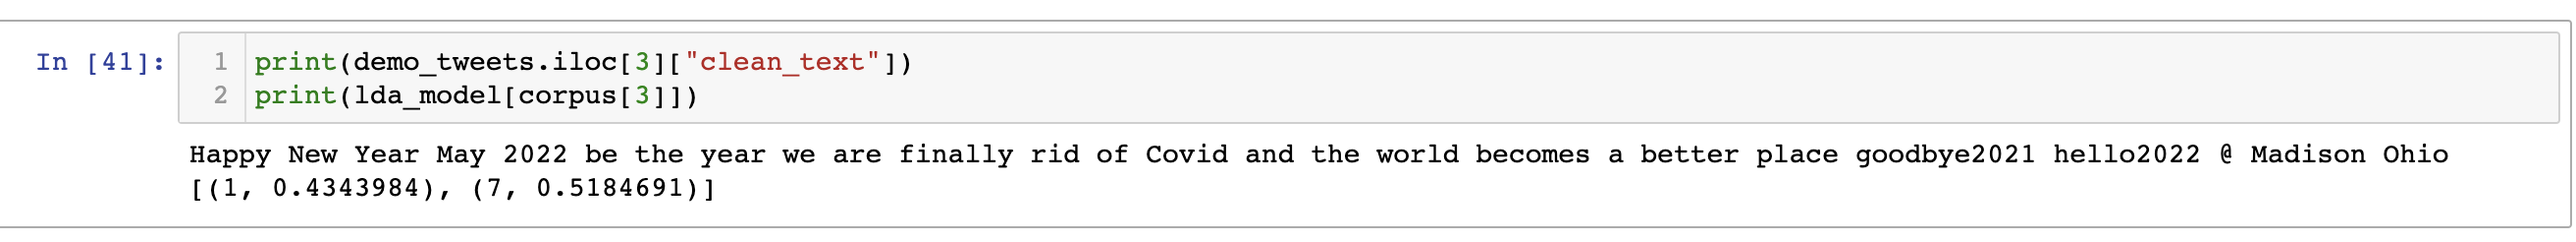
\includegraphics[width=0.5\textwidth]{imgs/infer.png}
    \caption{Result of inference on an unseen data point}
    \label{fig:infer}
\end{figure}
\begin{figure}[H]
    \centering
    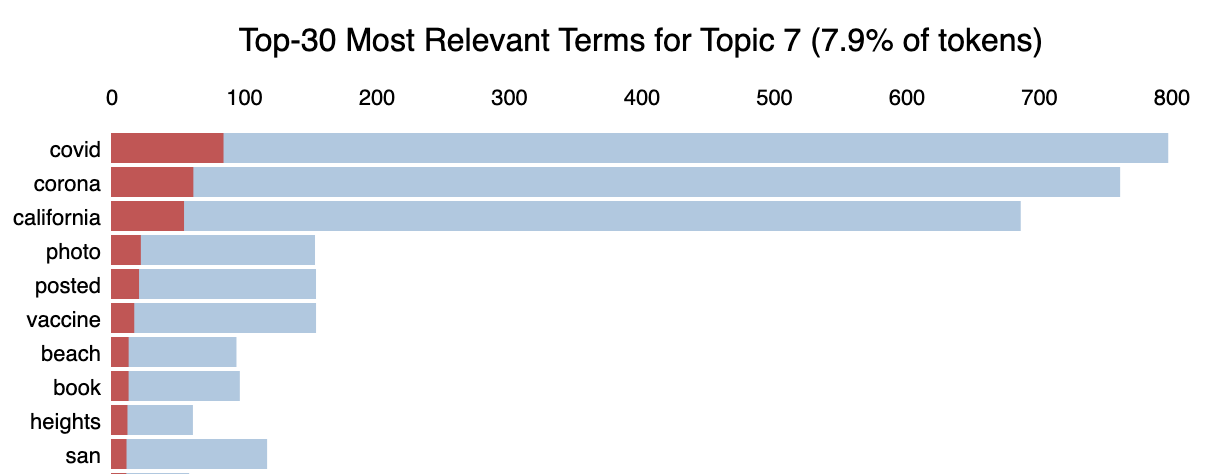
\includegraphics[width=0.5\textwidth]{imgs/cluster_7.png}
    \caption{Shows the term frequency for Topic Cluster 7}
    \label{fig:my_label}
\end{figure}
If we compare the sentiment score provided in the dataset, the value for the
corresponding data point is 0.3676 which falls inside a positive sentiment
score range.

\subsection{Spatial Data Mining and Visualization}
\subsubsection{Visualized image of data}
\begin{figure}[h]
\centering
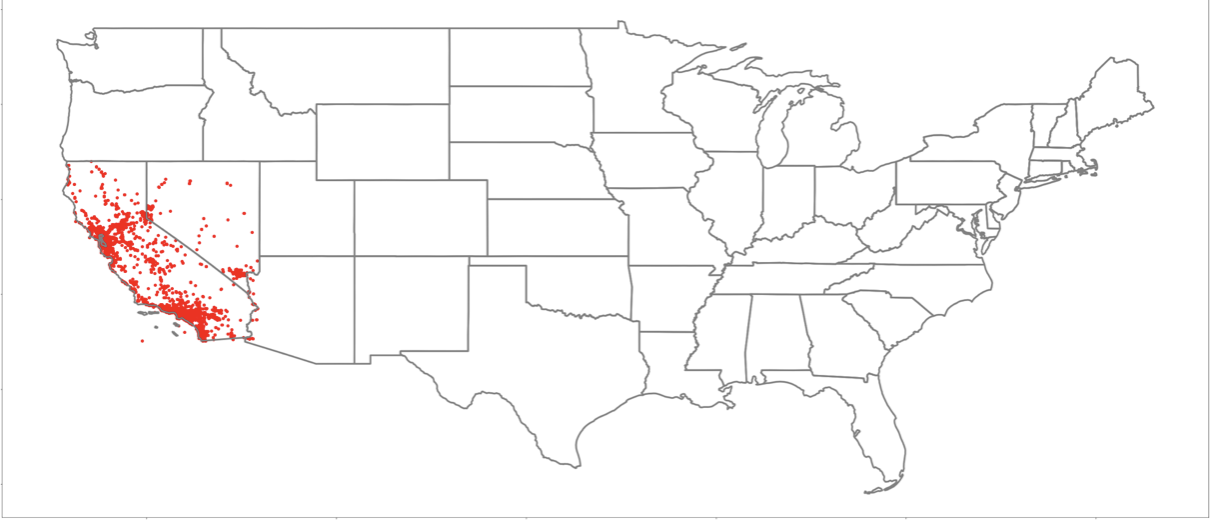
\includegraphics[width=0.5\textwidth]{imgs/USA.png}
\caption{\label{fig:Research process}Representation of unfiltered points on
 the continental United States map}
\end{figure}

This image above show the filtering result on envelope(minimum orthogonal
bounding rectangle) (Fig.14). By this method, we narrow down the geographic
range of the tweets and mark up them on the map. We can find that there are
some points outside of the state. Then we apply some spacial operator to
filter them (Fig.15).
\begin{figure}[h]
    \centering
    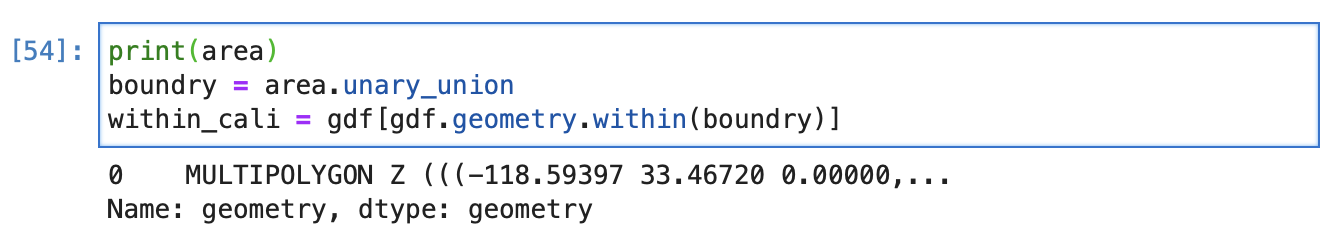
\includegraphics[width=0.5\textwidth]{imgs/sp_operator.png}
    \caption{\label{fig:Research process}Spatial operators}
\end{figure}
Then we get the result below, which contains only the points within this
state (Fig.16).
\begin{figure}[h]
    \centering
    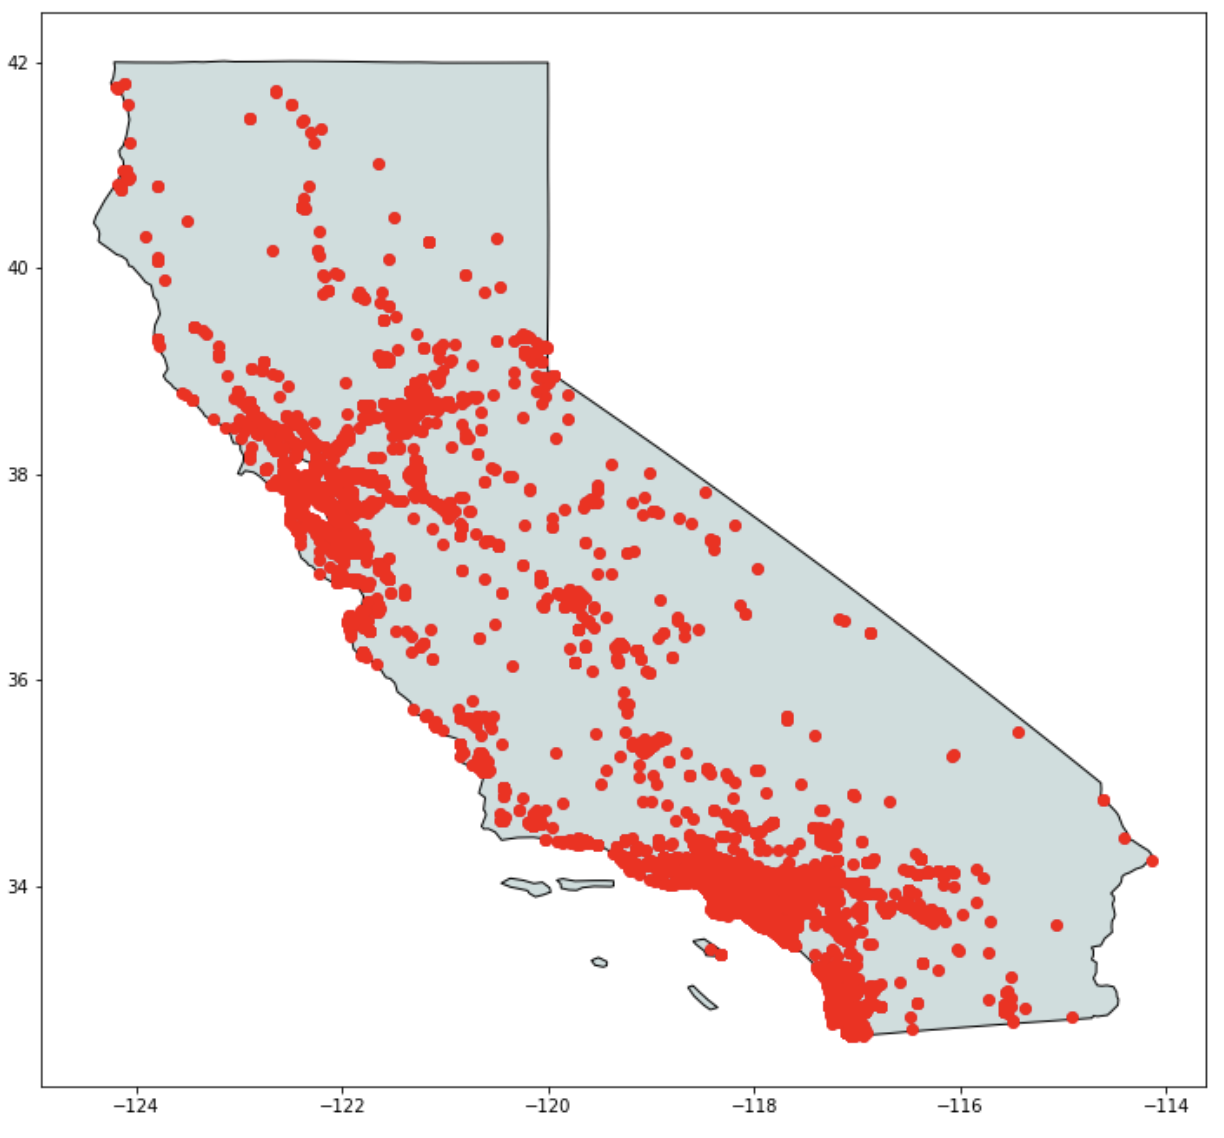
\includegraphics[width=0.4\textwidth]{imgs/ca1_result.png}
    \caption{\label{fig:Research process}Filtered dataset}
\end{figure}
We can also show the average of sentiment score distribution for the
Continental United States. The lighter the color, the more positive the
attitude of the district (Fig.17).
\begin{figure}[h]
    \centering
    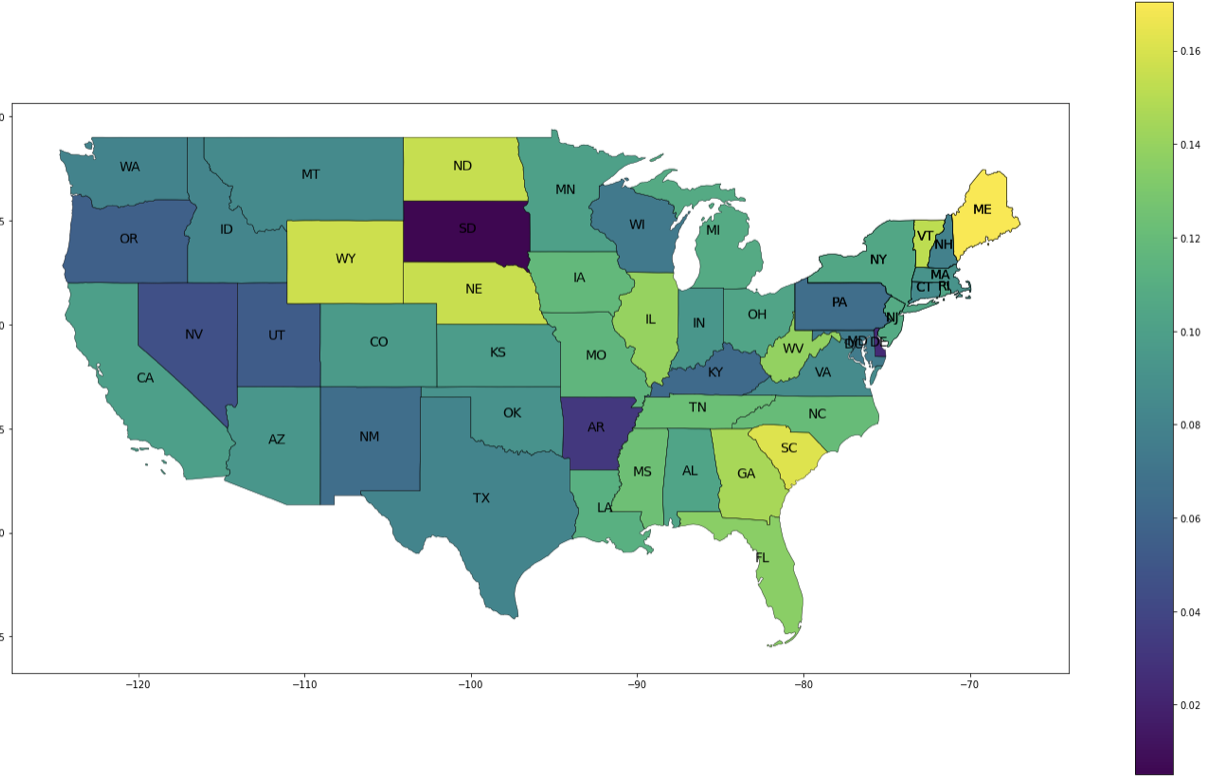
\includegraphics[width=0.5\textwidth]{imgs/USA_info.png}
    \caption{\label{fig:Research process}Color-coded sentiment index for each state}
\end{figure}
We can further subdivide the types of points. Red dots represent positive
tweets, while yellow dots represent negative tweets. We show the results for
several states. All of them are collected during July 2021 to February 2022.
The density of this point will be an important metrics for us to decide
whether we can use the dataset as the research object. If the number of
points is too small, the training result will be too random to reflect the
real tendency (Fig.18, 19, 20). 
\begin{figure}[h]
    \centering
    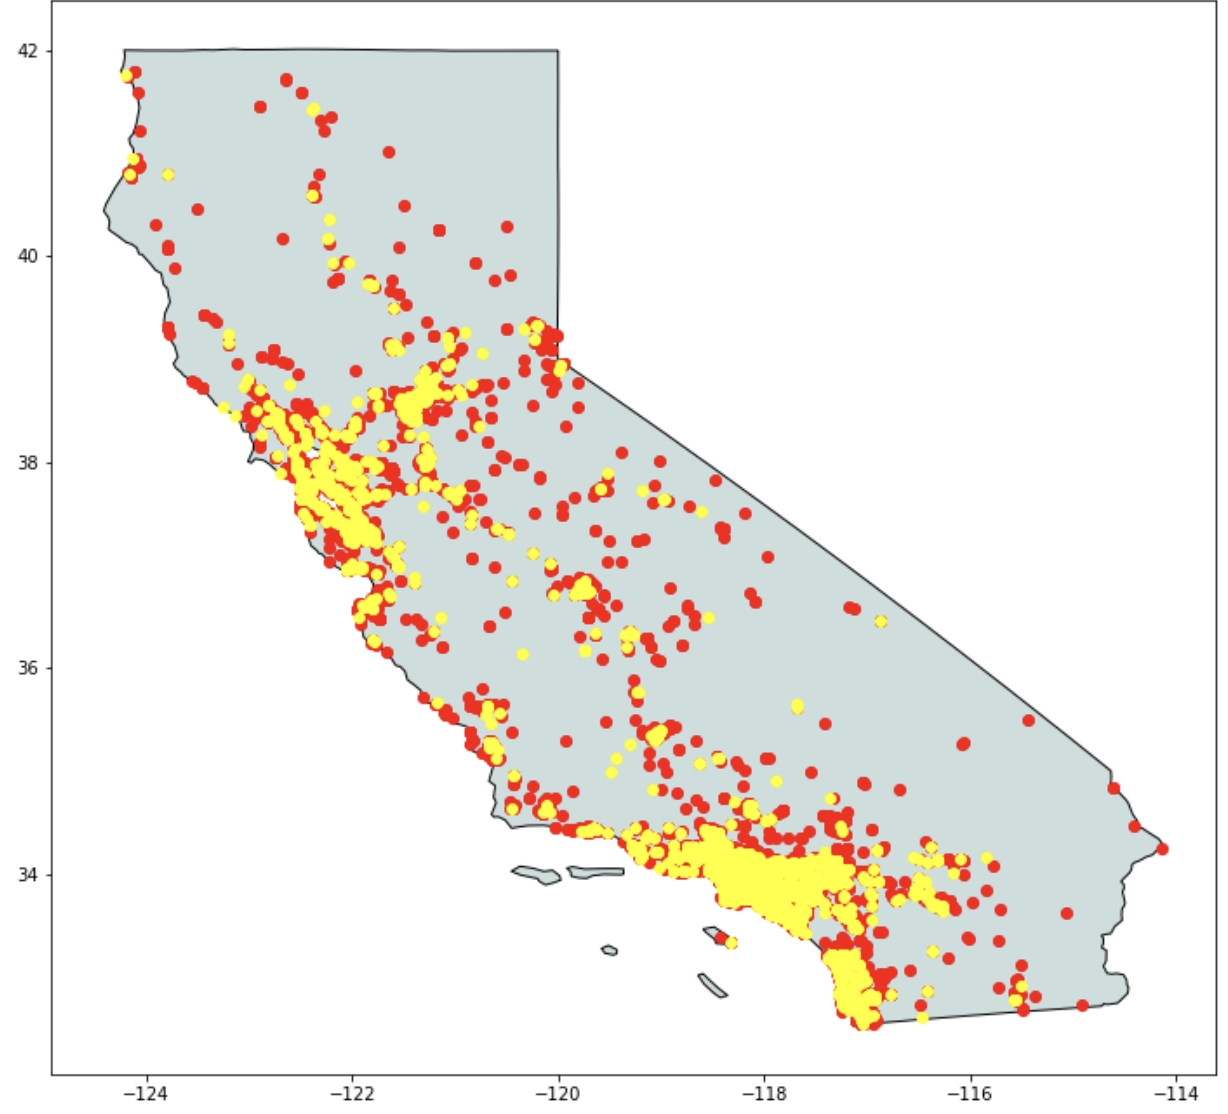
\includegraphics[width=0.4\textwidth]{imgs/CA.png}
    \caption{\label{fig:Research process}Distribution of tweets in California}
\end{figure}
\begin{figure}[h]
    \centering
    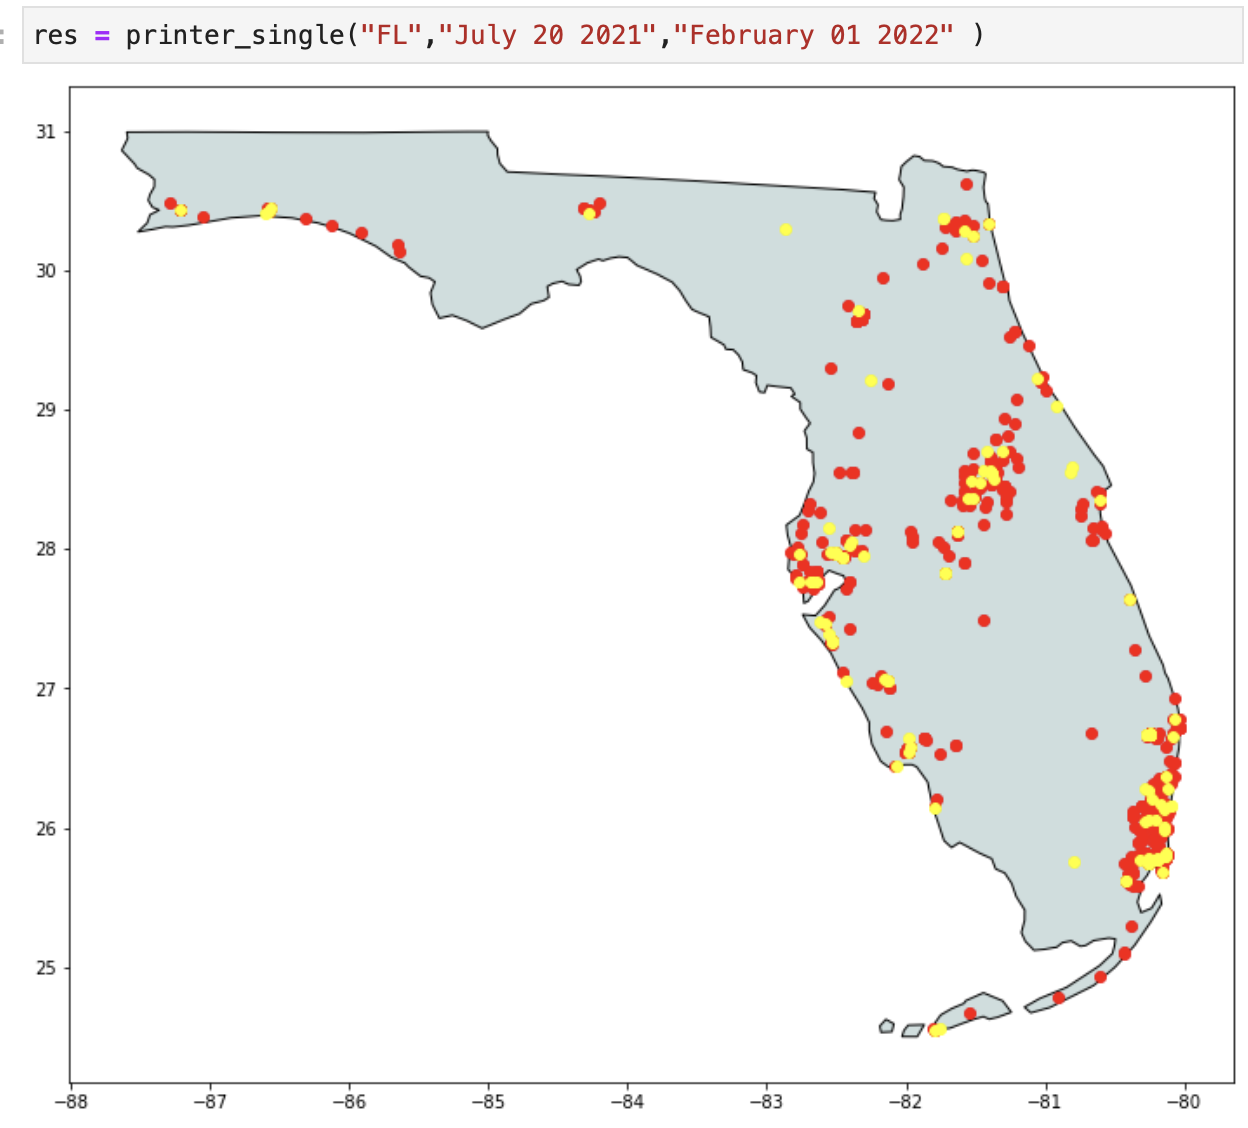
\includegraphics[width=0.4\textwidth]{imgs/FL.png}
    \caption{\label{fig:Research process}Distribution of tweets in Florida}
\end{figure}
\begin{figure}[h]
    \centering
    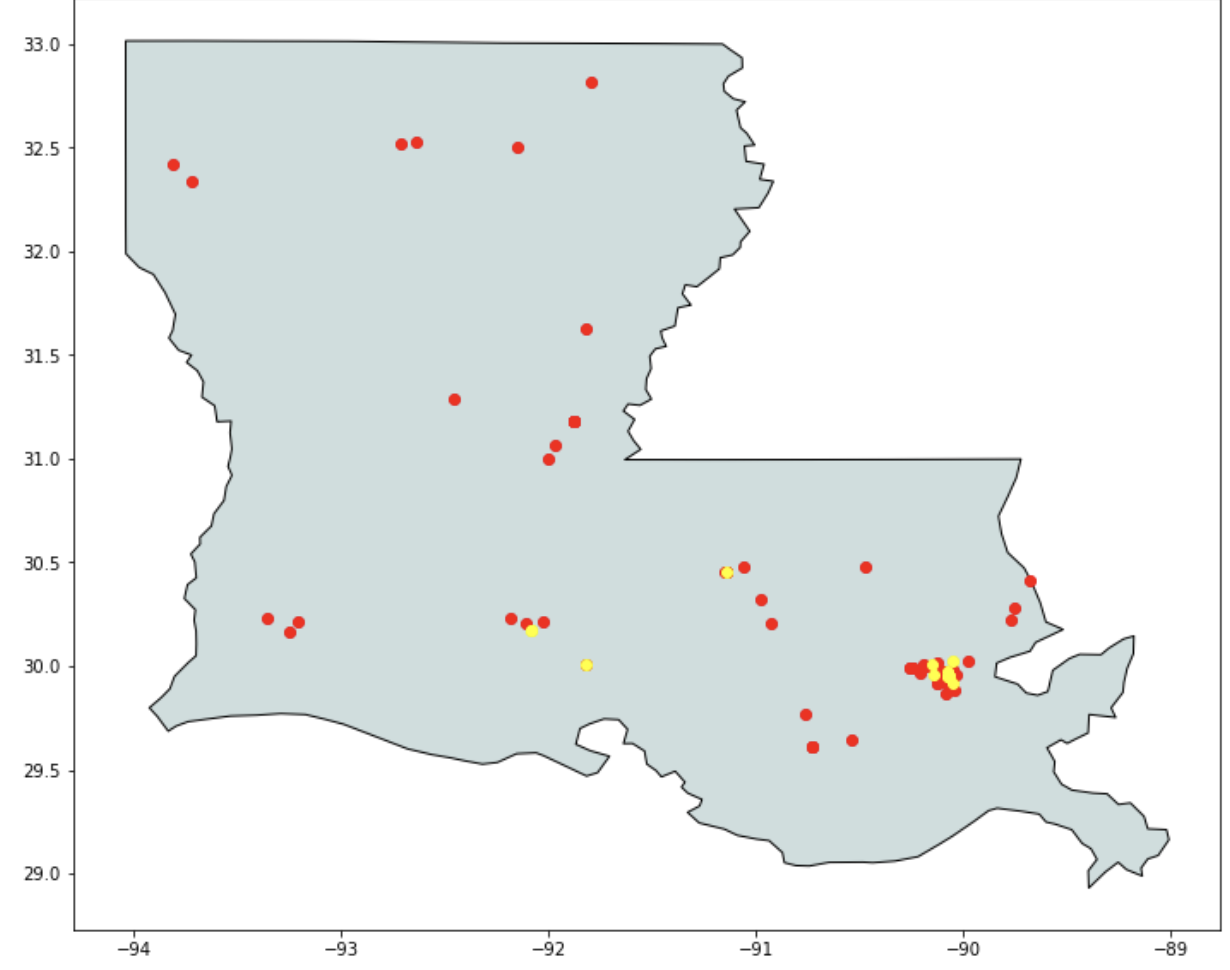
\includegraphics[width=0.4\textwidth]{imgs/LA.png}
    \caption{\label{fig:Research process}Distribution of tweets in Los Angeles}
\end{figure}